% --------------------------------------------------------------
% This is all preamble stuff that you don't have to worry about.
% Head down to where it says "Start here"
% --------------------------------------------------------------
 
\documentclass[12pt]{article}
 
\usepackage[margin=1in]{geometry} 
\usepackage{amsmath,amsthm,amssymb}
 
\newcommand{\N}{\mathbb{N}}
\newcommand{\Z}{\mathbb{Z}}
 
\newenvironment{theorem}[2][Theorem]{\begin{trivlist}
\item[\hskip \labelsep {\bfseries #1}\hskip \labelsep {\bfseries #2.}]}{\end{trivlist}}
\newenvironment{lemma}[2][Lemma]{\begin{trivlist}
\item[\hskip \labelsep {\bfseries #1}\hskip \labelsep {\bfseries #2.}]}{\end{trivlist}}
\newenvironment{exercise}[2][Exercise]{\begin{trivlist}
\item[\hskip \labelsep {\bfseries #1}\hskip \labelsep {\bfseries #2.}]}{\end{trivlist}}
\newenvironment{problem}[2][Problem]{\begin{trivlist}
\item[\hskip \labelsep {\bfseries #1}\hskip \labelsep {\bfseries #2.}]}{\end{trivlist}}
\newenvironment{question}[2][Question]{\begin{trivlist}
\item[\hskip \labelsep {\bfseries #1}\hskip \labelsep {\bfseries #2.}]}{\end{trivlist}}
\newenvironment{corollary}[2][Corollary]{\begin{trivlist}
\item[\hskip \labelsep {\bfseries #1}\hskip \labelsep {\bfseries #2.}]}{\end{trivlist}}

\newenvironment{solution}{\begin{proof}[Solution]}{\end{proof}}

\usepackage{lipsum}
\usepackage[colorlinks=true, linkcolor=blue, citecolor=blue, urlcolor=blue]{hyperref}
\usepackage{cleveref}
\usepackage{graphicx}
\usepackage{subcaption}
\usepackage{minted}


\begin{document}
 
% --------------------------------------------------------------
%                         Start here
% --------------------------------------------------------------
 
\title{CS324 Deep Learning\\ \textbf{Assignment 2}}
\author{Kuang Liang}

\maketitle

\begin{abstract}

For this assignment, I implemented, trained and tested an MLP, a CNN and an RNN based on PyTorch. In the report, I will explain how I implemented them and the experiments I conducted with them.

\end{abstract}

\section{MLP}

\subsection{NumPy MLP and PyTorch MLP}

In Task 1 and Task 2, I tested the NumPy MLP model and the PyTorch MLP model under the same setting. As expected, they achieved the same accuracy on the datasets generated by \texttt{sklearn.datasets.make\_moons} and \texttt{sklearn.datasets.make\_circles}, see \cref{fig:p1,fig:p2}.

\begin{figure}[htbp]
    \centering
    \begin{minipage}{0.45\textwidth}
        \centering
        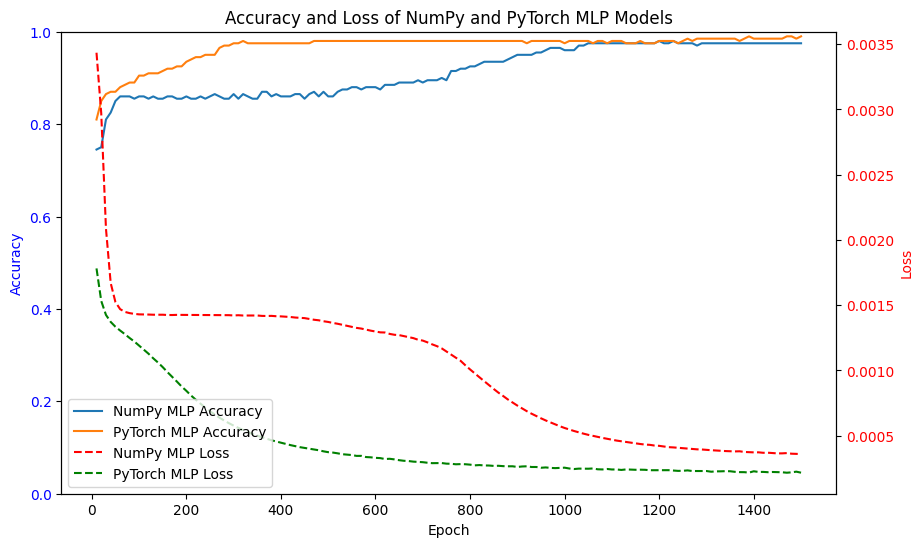
\includegraphics[width=\textwidth]{p1_fig1.png}
        \caption{\texttt{make\_moons} generator}
        \label{fig:p1}
    \end{minipage}%
    \hfill
    \begin{minipage}{0.45\textwidth}
        \centering
        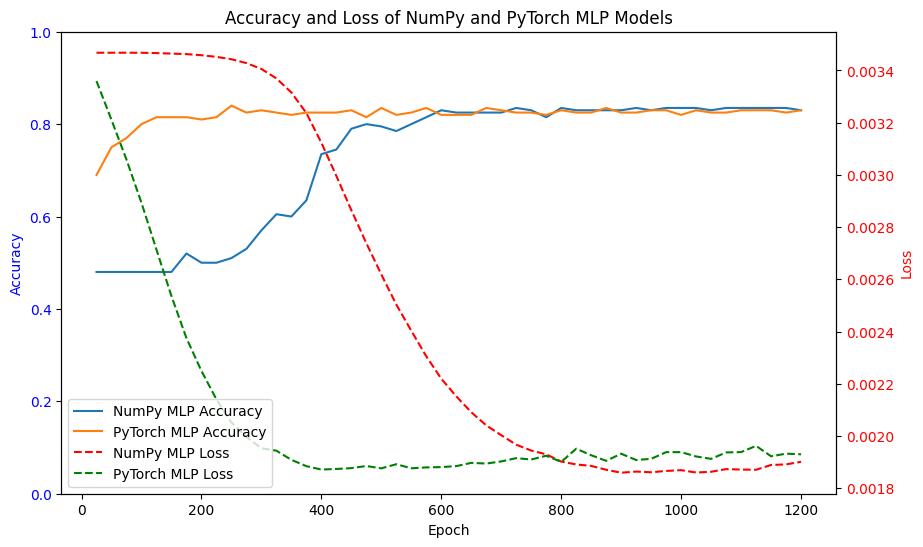
\includegraphics[width=\textwidth]{p1_fig2.png}
        \caption{\texttt{make\_circles} generator}
        \label{fig:p2}
    \end{minipage}
\end{figure}

\subsection{CIFAR-10 experiment on MLP}

In Task 3, I tried to achieve the best result on CIFAR-10 classification task with a self-defined MLPnet.

\subsubsection{Data preprocessing}

I have used several methods to preprocess the data\footnote{\texttt{transforms.ToTensor()} is emitted here as it is not for improving the performance.}.

\begin{itemize}
    \item [1.] \texttt{transforms.RandomHorizontalFlip()}: This randomly flips each image horizontally to augment the dataset by creating variations of the images.
    \item [2.] \texttt{transforms.RandomCrop(32, padding=4)}: This crops the image to a $32\times 32$ size with a padding of $4$ pixels, which adds randomness to the dataset by simulating slight shifts.
    \item [3.] \texttt{transforms.Normalize((0.4914, 0.4822, 0.4465), (0.2470, 0.2435, 0.2616))}: This normalizes the image tensor using the mean and standard deviation for each RGB channel, which are the computed means and standard deviations of the CIFAR-10 dataset\footnote{Parameters are from https://stackoverflow.com/questions/69747119}.
\end{itemize}

\subsubsection{Network design}

Also, I added some useful units to the MLP, see \cref{sec:Appendix_A}.

\begin{itemize}
    \item [1.] \texttt{nn.BatchNorm1d()}: This is the BN unit which reduces internal covariate shift.
    \item [2.] \texttt{nn.GELU()}: This is the Gaussian Error Linear Unit which nonlinearly amplifies values greater than zero, suppresses values less than zero, and is smoother than ReLU.
    \item [3.] \texttt{nn.Dropout()}: This randomly sets the output of some neurons in the neural network to zero, makes the model independent of specific neurons or feature combinations during training.
\end{itemize}

\subsubsection{Experiment}

I have done the ablation experiment of MLPnet on CIFAR-10, see \cref{tab:tab1}. Here, the MLP has the same linear layers as the MLPnet, and uses ReLU as the activation function. The preprocessing of data and the upgrading of the structure of the network improved the testing accuracy by 1.24\%.

\begin{table}[htbp]
    \centering
    \begin{tabular}{|c|c|c|}
        \hline
         Data Preprocessing & Model & Testing Accuracy \\ \hline
         w/o & MLP & 50.49 \\ \hline
         w/o & MLPnet & 50.44 \\ \hline
         w & MLP & 48.90 \\ \hline
         w & MLPnet & 51.73 \\ \hline
    \end{tabular}
    \caption{Ablation experiment of MLPnet on CIFAR-10.}
    \label{tab:tab1}
\end{table}

\section{CNN}

The CNN performs far better than the MLP, achieving an average testing accuracy of $83.30\%$ on CIFAR-10, mainly because of its ability to capture spacial information. The curve of validation accuracy and loss are shown in \cref{fig:p3}.

\begin{figure}
    \centering
    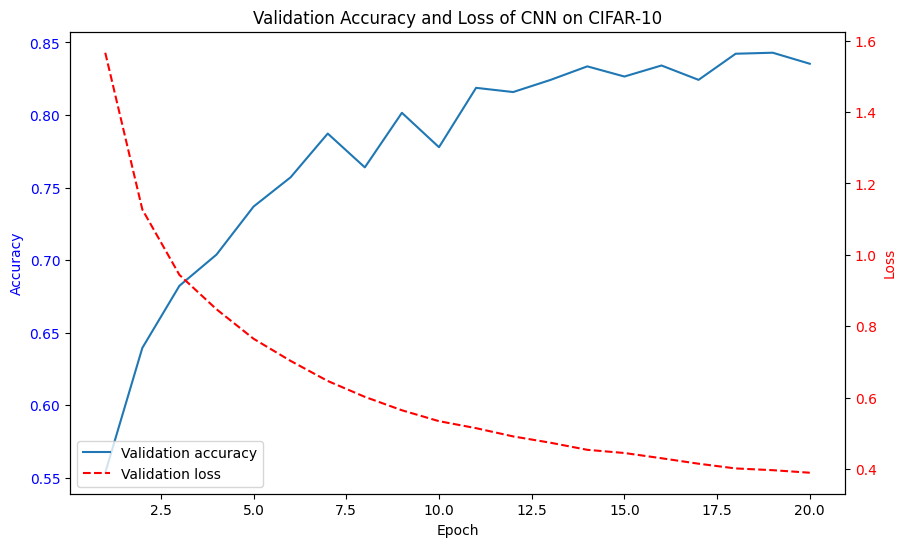
\includegraphics[width=0.5\linewidth]{p2_fig1.png}
    \caption{Validation Accuracy and Loss of CNN on CIFAR-10.}
    \label{fig:p3}
\end{figure}

\section{RNN}

I tested the RNN on the palindromic number dataset, see \cref{fig:p4}. The RNN is not perfectly stable on this task, and has a limited memory.

\begin{figure}
    \centering
    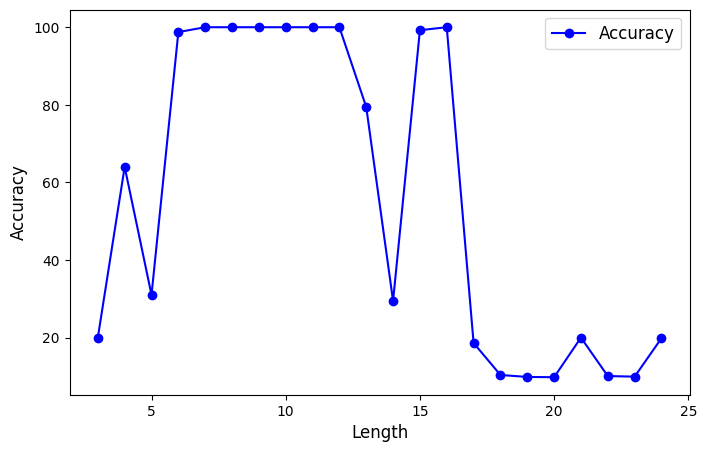
\includegraphics[width=0.5\linewidth]{p3_fig1.png}
    \caption{Validation Accuracy of RNN on palindromic number dataset of different lengths.}
    \label{fig:p4}
\end{figure}

\section{Conclusion}

Each of the three deep learning model is suited to a specific class of problems. MLP is used for general-purpose tasks, CNN is used for spatial data like images, and RNN is used for sequential data like time-series or language.

% \bibliographystyle{plain}
% \bibliography{main}

\newpage
\appendix

\section{MLP}
\label{sec:Appendix_A}

Here is how my MLPnet is defined in python.

\begin{minted}[fontsize=\small, linenos, frame=lines]{python}
import torch.nn as nn
class MLPnet(nn.Module):
    def __init__(self, input_size=3 * 32 * 32, num_class=10):
        super(MLPnet, self).__init__()
        self.model = nn.Sequential(
            nn.Flatten(),
            nn.Linear(input_size, 512),
            nn.BatchNorm1d(512),
            nn.GELU(),
            nn.Linear(512, 512),
            nn.BatchNorm1d(512),
            nn.GELU(),
            nn.Linear(512, 256),
            nn.BatchNorm1d(256),
            nn.GELU(),
            nn.Linear(256, 256),
            nn.BatchNorm1d(256),
            nn.GELU(),
            nn.Linear(256, 128),
            nn.BatchNorm1d(128),
            nn.GELU(),
            nn.Dropout(p=0.5)
        )
        self.classifier = nn.Linear(128, num_class)
    def forward(self, x):
        feature = self.model(x)
        out = self.classifier(feature)
        return out
\end{minted}

% --------------------------------------------------------------
%     You don't have to mess with anything below this line.
% --------------------------------------------------------------
 
\end{document}
